%%%%%%%%%%%%%%%%%%%%%%%%%%%
% PREAMBOLO DEL DOCUMENTO %
%%%%%%%%%%%%%%%%%%%%%%%%%%%
\documentclass[a4paper,11pt,oneside,top=3cm,bottom=3cm,left=3.5cm,right=3.5cm,openright,reqno,table]{book}

% openany - fa iniziare i capitoli direttamente nella pagina successiva
% openright - fa iniziare i capitoli nella prima pagina destra disponibile 
% fleqn  - allinea le formule a sinistra anzichè centrarle
% leqno - dispone la numerazione delle formule sulla sinistra o destra
% reqno - dispone la numerazione delle formule sulla destra
%
\usepackage{packages}
% Per non appesantire troppo questo file
% quasi tutti i pacchetti usati sono salvati in packages.sty
%
\linespread{1.5}
% Per avere la parola BOZZA scritta su tutte le pagine

% funziona solo in modalità PS
% Invece per i PDF ho risolto così:
% pdftk tesi.pdf background bozza.pdf output tesi_bozza.pdf
%
%%%%%%%%%%%%%%%%%%%%%%%%%%%%%%%%%
%   DOCUMENTO VERO E PROPRIO    %
%%%%%%%%%%%%%%%%%%%%%%%%%%%%%%%%%
\begin{document}
% FRONTESPIZIO %
\begin{titlepage}
\changepage{}{}{}{-7.5 mm}{}{}{}{}{}
% parametri per cambiare le dimensioni di una singola pagina in ordine:
% {textheight}{textwidth}{evensidemargin}{oddsidemargin}{columnsep}
% {topmargin}{headheight}{headsep}{footskip}
% se voglio centrare la pagina devo mettere bindingoffset/2
% i primi 5 parametri posso usarli con \changetext


\begin{center}

\includegraphics [width=.15\columnwidth, angle=0]{unisa}\\ % height
\vspace{0.5cm}
{\LARGE \scshape Università degli Studi di Salerno}\\
\vspace{0.5cm}
{\Large Dipartimento di Informatica}\\
\vspace{0.1cm}
{\large Corso di Laurea Triennale in Informatica}\\
\vspace{1.5cm}
{\Large \scshape Tesi di Laurea} \\
\vspace{4cm}
{\Huge \bfseries TITOLO TESI} \\
\vspace{5cm}

\begin{minipage}[t]{7cm}
\flushleft
\textsc{Relatore}

Prof. \textbf{Andrea De Lucia} \\
{\small Università degli studi di Salerno} \\[0.25cm]
\end{minipage}
\hfill
\begin{minipage}[t]{7cm}
\flushright
\textsc{Candidato}

\textbf{Nome Cognome} \\
Matricola: 0123456789
\end{minipage}

\vspace{3cm}

%& & \\
%& Candidato & \\
%& \textbf{Fabiano Pecorelli} & \\
{\small Anno Accademico YYYY-YYYY} %\\
%
%
\begin{comment}
\begin{table}[!h]
\centering
\begin{tabular}{c c c} %p{5cm}c
& Tesi di laurea & \\
& \textbf{Fabiano Pecorelli} & \\
& & \\[0.25cm]
Relatore \\
prof. \textbf{Andrea De Lucia} \\
{\small Università degli studi di Salerno} & & {\small Provincia di Salerno}\\
& & \\[0.5cm]
& {\small A.A. 2015-2016} & \\
\end{tabular}
\end{table}
\end{comment}
%
%
\end{center}

\end{titlepage}
%

\frontmatter
% quello che segue è in numerazione romana e i capitoli non verranno numerati
% se non si vuole che compaia il numero di pagina basta usare il comando:
%\nonumber

% RINGRAZIAMENTI %
\begin{titlepage}

\nonumber
\null \vspace {\stretch{1}}
	\begin{flushright}
%	\begin{verse}
\textit{INSERIRE QUI UNA DEDICA O UNA CITAZIONE} \\[5mm]
%	\end{verse}
	\end{flushright}



\end{titlepage}
% SOMMARIO %
\cleardoublepage
%\selectlanguage{italian}
\begin{abstract}

    Il contesto applicativo della tesi è incentrato sullo studio di tecniche di Intelligenza Artificiale applicate al gioco degli scacchi, trattate in due diversi moduli. Nel primo modulo è stato considerato il problema della ricerca della mossa migliore nel corso di una partita, risolto attraverso algoritmi di Intelligenza Artificiale dei quali è stata fornita un'analisi delle prestazioni da un punto di vista computazionale. Nel secondo modulo è stato creato e addestrato un modello di rete neurale capace di giocare autonomamente a scacchi, del quale è stato stimato un punteggio che ne indica la performance sportiva.
\\[1cm]
\end{abstract} 
% INDICI %
\phantomsection
\addcontentsline{toc}{chapter}{Indice}
\tableofcontents
% Il simbolo * serve per evitare che comapaia nell'indice
\clearpage
%\listoffigures
%\clearpage
%\listoftables
% GLOSSARIO
%\cleardoublepage
\phantomsection
\addcontentsline{toc}{chapter}{Glossario}
% per inserire l'elenco dei simboli e degli acronimi nell'indice
\printglossary
% Per stampare il glossario
% per aggiornarlo si deve eseguire da terminale:
% makeindex -s myDoc.ist -t myDoc.alg -o myDoc.acr myDoc.acn
% per inserire una voce nell'elenco:
% \newglossaryentry{voce_etichetta}{name={voce}, description={descrizione}}
% se non compare direttamente nel testo va inizializzata con:
% \glsadd{voce_etichetta}
% oppure se viene richiamata all'interno del testo:
% \gls{voce_etichetta}
% SIMBOLI E NOTAZIONI %
\cleardoublepage
\phantomsection
\addcontentsline{toc}{chapter}{Elenco delle figure}
% per inserire l'elenco dei simboli e degli acronimi nell'indice
%\printglossary[type=\acronymtype,title=Elenco delle figure]
% Per stampare l'elenco dei simboli
\listoffigures
\cleardoublepage
\phantomsection
\addcontentsline{toc}{chapter}{Elenco delle tabelle}
% per inserire l'elenco dei simboli e degli acronimi nell'indice
%\printglossary[type=\acronymtype,title=Elenco delle figure]
% Per stampare l'elenco dei simboli
\listoftables
% per aggiornarlo si deve eseguire da terminale:
% makeindex -s myDoc.ist -t myDoc.glg -o myDoc.gls myDoc.glo
% per inserire una voce nell'elenco:
% \newglossaryentry{voce_etichetta}{name={voce}, description={descrizione}}
% se non compare direttamente nel testo va inizializzata con:
% \glsadd{voce_etichetta}
% oppure se viene richiamata all'interno del testo:
% \gls{voce_etichetta}

\mainmatter
% quello che segue sarà in numerazione araba e i capitoli verranno numerati
%\part{Studio iniziale}
% CAPITOLI
\phantomsection
%\addcontentsline{toc}{chapter}{Introduzione}
\chapter{Introduzione}
\section{Contesto applicativo}
Lo studio proposto è incentrato sulla disciplina degli scacchi. Nello specifico vengono passate a rassegna diverse tecniche di 
Intelligenza Artificiale volte a ricercare (e compiere) una mossa valida sulla scacchiera nel corso di una partita regolare.
Vengono resi noti i due differenti approcci adottati per il conseguimento degli obiettivi sopracitati: 
\begin{itemize}
    \item \textbf{Primo approccio}: dei "semplici" algoritmi di ricerca valutano lo stato corrente della scacchiera ed effettuano una 
    possibile mossa;
    \item \textbf{Secondo approccio}: viene addestrato un modello di Intelligenza Artificiale che impari a giocare simulando le 
    mosse di un giocatore umano. 
\end{itemize}
\markboth{Introduzione}{}
% [titolo ridotto se non ci dovesse stare] {titolo completo}

\section{Motivazioni e Obiettivi} %\label{1sec:scopo}
Fra i giochi più popolari al mondo, gli scacchi possono essere giocati ovunque (all'aperto, in circolo, online) e la vastità del numero di 
giocatori è stata tale da favorire lo sviluppo di diverse Federazioni (tra le quali, la più importante, la 
\textbf{Fédération Internationale des Échecs - FIDE}) con conseguenti tornei e competizioni in tutto il mondo. 
Le motivazioni della stesura del presente elaborato sono da ricercare nella natura intrinseca del gioco stesso. Gli scacchi rientrano
tra i giochi di strategia più complessi da padroneggiare, con un numero di mosse esponenzialmente elevato ($10^{123}$) rendendo il numero 
di partite pari a circa $10^{10^{50}}$. Gli obiettivi finali sono dunque da ricercare nelle motivazioni stesse; la vera protagonista del
presente lavoro di tesi è infatti la \textbf{complessità} del gioco degli scacchi, che viene analizzata, studiata e approfondita nei paragrafi
seguenti, non senza un'attenta critica e analisi accurata sui risultati raggiunti.

\section{Risultati}
%da revisionare
Gli algoritmi di ricerca e di apprendimento sfruttati nei due diversi moduli offrono una panoramica generale sulle moderne tecniche di intelligenza
artificiale che non solo vengono applicate al giorno d'oggi ma sono in continua evoluzione. I risultati ottenuti non vogliono aprire nuovi
orizzonti a differenti approcci sullo studio, ma fanno più da panoramica generale a tecniche già esistenti.

\section{Struttura della tesi}
La trattazione del lavoro di tesi è strutturata secondo il seguente elenco:
\begin{itemize}
    \item \textbf{Introduzione}: viene fornita una panoramica dello studio effettuato, con particolare attenzione alle motivazioni, 
    agli obiettivi e ai risultati del lavoro svolto.
    \item \textbf{Stato dell'arte}: l'attenzione viene spostata sulle tecnologie e tecniche adottate in uno specifico contesto.
    \item \textbf{Design}: si esaminano nel dettaglio la progettazione e l'implementazione del lavoro.
    \item \textbf{Conclusioni}: vengono presentate riflessioni e considerazioni di carattere generale con eventuali riferimenti
    agli sviluppi futuri.
\end{itemize}

\chapter{Ruolo del gioco degli scacchi nell'Intelligenza Artificiale} %\label{1cap:spinta_laterale}
% [titolo ridotto se non ci dovesse stare] {titolo completo}
%
\begin{citazione}
    Questo capitolo illustra lo stato dell'arte e i lavori presenti in letteratura sugli aspetti di ricerca trattati nel nostro studio. 
    Prima di dare un'occhiata alla varietà degli approcci adottati per affrontare il problema della complessità degli scacchi, è opportuno fare un passo indietro per capire meglio di \textit{che cosa} si parla.
\end{citazione}
\section{Teoria dei giochi}
La \textbf{teoria dei giochi}\cite{colombo2003introduzione} è una branca della matematica che studia l'interazione strategica tra gli individui nell'ambito di un \textbf{gioco}. In questo senso viene considerato gioco uno scenario in cui i contendenti (giocatori) seguono un determinato tipo di comportamento (strategia) al fine di massimizzare la propria vincita. Nel complesso l'esito finale del gioco coincide con il risultato della sequenza delle strategie adottate dai giocatori e dai loro avversari. Chiarito lo scopo e il significato dei giochi, questi vengono divisi in 5 gruppi principali:
\begin{itemize}
    \item \textbf{giochi cooperativi e non cooperativi}: nei giochi cooperativi i giocatori possono formare alleanze per massimizzare le probabilità di vincita. Ciò non è possibile nei giochi non cooperativi;
    \item \textbf{giochi simmetrici e asimmetrici}: nei giochi simmetrici tutti i partecipanti hanno gli stessi obiettivi, ed è fondamentale elaborare strategie vincenti. Nei giochi asimmetrici, invece, i giocatori hanno obiettivi diversi;
    \item \textbf{giochi ad informazione perfetta e ad informazione imperfetta}: nei giochi ad informazione perfetta tutti i giocatori possono vedere le mosse degli altri giocatori. Le mosse sono invece nascose nei giochi ad informazione imperfetta;
    \item \textbf{giochi simultanei e sequenziali}: nei giochi simultanei i giocatori possono giocare le proprie mosse simultaneamente, piuttosto che a turni come avviene nei giochi sequenziali;
    \item \textbf{giochi a somma zero e a somma non zero}: nei giochi a somma zero la vincita di un giocatore è equilibrata dalla perdita di un altro. Nei giochi a somma non zero, invece, più giocatori possono trarre vantaggio dalle vincite di un altro.
\end{itemize}
Il gioco degli scacchi è pertanto considerato un gioco non cooperativo e simmetrico, poiché le partite sono solitamente disputate tra due singoli avversari che puntano entrambi a vincere la partita. Ciascun giocatore è tenuto a muovere i propri pezzi a turno davanti agli occhi dell'avversario, e alla fine della partita la vincita di un giocatore comporta la perdita dell'altro: queste caratteristiche rendono gli scacchi un gioco ad informazione perfetta, sequenziale e a somma zero. 
\subsection{Teoria dei giochi e Intelligenza Artificiale}
I giochi ritenuti più interessanti nell'ambito dell'Intelligenza Artificiale sono quelli \textbf{a somma zero} con \textbf{informazione perfetta}, solitamente a turni e a due giocatori. Le azioni degli agenti sono pertanto sequenziali, e le loro funzioni di utilità alla fine della partita sono uguali ma di segno opposto (vittoria +1, sconfitta -1). I primi approcci dell'Intelligenza Artificiale allo studio dei giochi si ebbero già nel 1950 proprio con gli scacchi. Da quel punto in poi le macchine hanno pian piano superato le capacità degli esseri umani anche nella dama in molti altri giochi. L'interesse verso i giochi è dovuto alla \textbf{facilità} nella loro rappresentazione contrapposta alla \textbf{difficoltà} nel risolverli\cite{russell2005intelligenza}. Un gioco può infatti essere definito come un \textbf{problema di ricerca} avente le seguenti caratteristiche:
\begin{itemize}
    \item lo \textbf{stato iniziale}, che specifica la configurazione di partenza del gioco stesso;
    \item il \textbf{giocatore} a cui tocca fare una mossa in un dato stato;
    \item l'\textbf{insieme delle mosse} lecite in un determinato stato;
    \item il \textbf{modello di transizione} cioè il risultato di una mossa;
    \item il \textbf{test di terminazione} che controlla se la partita è finita oppure no;
    \item la \textbf{funzione obiettivo} che definisce il valore numerico finale per un gioco che termina in un particolare state per un particolare giocatore.
\end{itemize}
L'\textbf{obiettivo} principale nello studio di questi problemi è dunque la ricerca di una strategia da adottare considerando le mosse dell'avversario; più in particolare si ricerca una strategia \textbf{ottima} che porti ad un risultato almeno pari a quello di qualsiasi altra strategia, assumendo che si stia giocando contro un giocatore infallibile. Tale ricerca si traduce nella visita dell'\textbf{albero di gioco}, ossia un albero in cui i nodi sono stati del gioco e gli archi le mosse. La visita dell'albero delle mosse del gioco degli scacchi è rimandata al Capitolo \ref{cap: design}. Prima di parlare delle soluzioni proposte al problema degli scacchi è opportuno comprendere a fondo le regole che vengono tutt'oggi osservate nelle partite.
\section{Come si gioca a scacchi}
\subsection{Preparazione della scacchiera}
Le regole ufficiali del gioco degli scacchi\cite{lawsofchess} prevedono che la scacchiera sia inizialmente disposta in modo che ogni giocatore abbia una casella chiara nell'angolo inferiore destro. Ai due angoli opposti sono collocate le due torri, seguite dai due cavalli e dai due alfieri. La regina occupa sempre la casella del proprio colore, e il re è collocato accanto alla regina. Tutta la seconda traversa è invece occupata dai pedoni.
\begin{figure}[!htb]
    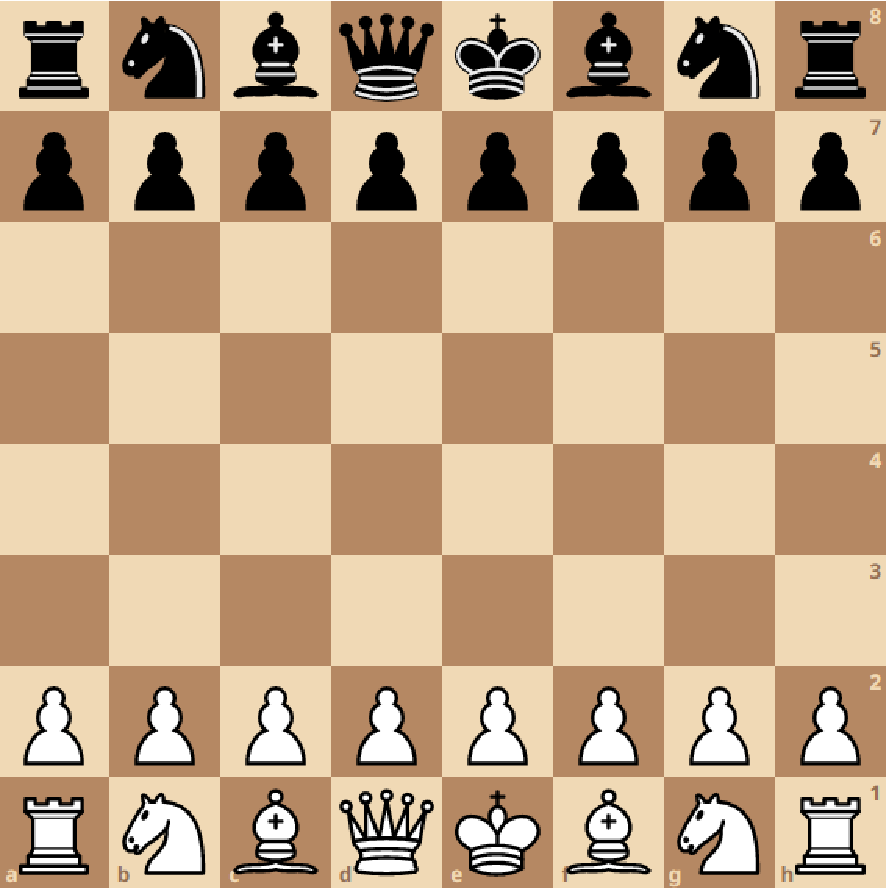
\includegraphics[width=10cm]{frontmatter/figure/scacchiera_iniziale.pdf}
    \centering
    \caption{Disposizione dei pezzi all'inizio della partita}
    \label{fig:checkmate}
\end{figure}
\subsection{Come si muovono i pezzi}
Ogni tipologia di pezzo segue delle regole ben precise nei movimenti. Non è possibile, ad esempio, muovere dei pezzi attraversando altri pezzi (eccetto per il cavallo, che può "saltarli") e ogni casella può essere occupata soltanto da un pezzo per volta. Negli scacchi è possibile liberare una casella dall'occupazione avversaria, \textbf{catturando} il pezzo interessato ed eliminandolo dalla scacchiera fino alla fine della partita. Come accennato in precedenza, ogni pezzo si muove in modo diverso dall'altro. In particolare:
\begin{itemize}
    \item il \textbf{re} può muoversi soltanto di una casella per volta nelle 8 direzioni disponibili, ma non è possibile spostarlo in una casella che lo metterebbe sotto \textbf{scacco} (minacciato da un pezzo avversario);
    \item la \textbf{regina} può muoversi in qualsiasi direzione seguendo una linea retta sia in orizzontale che in diagonale di quante caselle vuole. Come tutti gli altri pezzi, in caso di cattura di un pezzo avversario il suo movimento si conclude nella casa precedentemente occupata dal pezzo catturato;
    \item la \textbf{torre} può muoversi di quante caselle si desidera, ma soltanto in avanti, indietro e di lato. Le due torri, quando ben collegate, si proteggono a vicenda e risultano estremamente utili;
    \item l'\textbf{alfiere} può muoversi in diagonale, e in virtù di questa caratteristica ogni alfiere rimane sullo stesso colore fino alla fine della partita (uno sulle caselle chiare e l'altro sulle caselle scure);
    \item il \textbf{cavallo} segue dei movimenti "a L", avanzando di due caselle in una direzione e poi di un'altra casella a 90°;
    \item il \textbf{pedone} può muoversi di una sola casella in avanti (oppure anche due se è la sua prima mossa), ma cattura i pezzi avversari in diagonale di una casella. Non è possibile indietreggiare, né catturare all'indietro. Inoltre, se un pedone raggiunge il lato opposto della scacchiera può trasformarsi in qualsiasi altro pezzo.
\end{itemize}
Negli scacchi è possibile effettuare l'\textbf{arrocco}: si tratta di una mossa speciale che consente non solo di mettere il proprio re al sicuro, ma anche di sviluppare una torre portandola in gioco. Per effettuare l'arrocco si sposta il re di due case verso destra o sinistra e si sposta la torre di una casella accanto al re, ma in direzione opposta. Tuttavia, non è possibile effettuare l'arrocco se il re o la torre in questione siano già stati mossi in un turno precedente, o se le caselle interessate nell'arrocco siano occupate da altri pezzi o controllate da pezzi avversari. 
Un'altra regola speciale degli scacchi riguarda la cattura \textbf{en passant} dei pedoni: se un pedone muove di due case alla sua prima mossa portandosi accanto a un pedone avversario (saltando la casella su cui sarebbe stato catturato), l'avversario ha la possibilità di catturare quel pedone occupando la casella aventi in diagonale. Questa speciale cattura deve però essere effettuata nel turno immediatamente successivo all'avanzamento del pedone, altrimenti non sarà più possibile farlo.
Nel gioco degli scacchi, è \textbf{sempre} il giocatore con i pezzi bianchi a muovere per primo. Questo privilegio porta un leggero vantaggio al bianco, che nella maggior parte dei casi imposterà piani d'attacco e di difesa già dalla prima mossa.

\subsection{Vincere una partita a scacchi}
L'obiettivo del gioco degli scacchi è quello di attaccare il re avversario, cercando di impedirgli di sottrarsi alla minaccia. Esistono, infatti, tre modi per difendere il proprio re da uno scacco: spostandolo in una casella libera e non minacciata, interponendo un proprio pezzo oppure catturando il pezzo che minaccia il re. Se il re non può liberarsi dallo scacco in nessuno dei tre modi, la partita viene dichiarata finita per \textbf{scacco matto}. Esistono casi in cui una partita di scacchi si conclude con una \textbf{patta}, cioè in parità, senza vincitori. Ciò accade principalmente per 5 motivi:
\begin{itemize}
    \item tutti i propri pezzi sono stati catturati, tranne il re. Non è possibile eseguire alcuna mossa legale, ma contemporaneamente il re non è sotto scacco. In questo caso, la partita finisce per \textbf{stallo}:
    \item i giocatori possono semplicemente accordarsi e smettere di giocare;
    \item non è possibile dare scacco matto in alcun modo (per esempio, un re e un alfiere contro un re);
    \item è stata ripetuta la stessa posizione per la terza volta nel corso della partita;
    \item sono state giocate 50 mosse consecutive senza catturare alcun pezzo.
\end{itemize}
\section{Breve panoramica sui motori scacchistici}
\subsection{Turochamp}
Come accennato nel capitolo \ref{cap: introduzione}, la complessità degli scacchi è ciò che li rende una delle sfide più interessanti 
dell'Intelligenza Artificiale. Alan Turing, uno dei padri dell'informatica, fu tra i primi ad interessarsi in maniera concreta al problema, progettando 
\textit{Turochamp}\footnote{Ideato nel 1948, \textit{Turochamp} nacque ben prima di un calcolatore che fosse in grado di 
leggere ed eseguire il programma. Ciò portò lo stesso Turing a valutare la "bontà" dell'algoritmo, analizzando le mosse con carta e penna.}, un algoritmo per giocare a scacchi\cite{godena2021eterna}.
La sua debolezza fu però evidenziata da Garri Kasparov in una conferenza del 2012, che mostrò che l'algoritmo era 
in grado di valutare un numero molto limitato di varianti\cite{kasparov2017reconstructing}. Il contributo di \textit{Turochamp}, in ogni caso, gettò delle importanti basi 
per l'evoluzione delle moderne tecniche di ricerca minimax.

\subsection{Deep Blue}
Fu solo nel 1996 che si cominciarono a temere le enormi potenzialità dei computer in ambito scacchistico: in quell'anno fu disputata 
una partita in condizioni normali di torneo tra Kasparov (allora campione del mondo) e \textit{Deep Blue}, un computer progettato 
da IBM appositamente per giocare a scacchi. La partita si concluse con l'abbandono da parte del campione dopo 40 mosse. Nel 1997, in occasione della rivincita, 
Kasparov abbandonò dopo sole 19 mosse\footnote{Alcune mosse di \textit{Deep Blue} risultarono a Kasparov piuttosto creative e incomprensibili,
al punto da sospettare che la macchina stesse ricevendo un supporto umano nel corso della partita. Effettivamente il codice del programma 
fu modificato tra una sfida e l'altra, permettendo alla macchina di non cadere nelle trappole del campione nelle mosse finali della partita.}. 
Questi eventi aprirono le basi ai moderni motori scacchistici, che nel corso degli anni hanno dimostrato di saper tener testa anche 
ai migliori giocatori di scacchi\cite{newborn2012kasparov}.
La potenza computazionale di \textit{Deep Blue} era dovuta al \textbf{parallelismo massivo}: furono utilizzati ben 480 processori (progettati per il gioco degli 
scacchi), che eseguivano un algoritmo scritto in linguaggio C in grado di calcolare 200 milioni di posizioni al secondo. Le funzioni di 
valutazione erano scritte in forma generale, mentre la lista delle aperture fu fornita dai campioni Illescas, Fedorowicz e De Firmian.

\subsection{Stockfish}
\textit{Stockfish} è un motore scacchistico open-source considerato uno dei più forti in assoluto. Correntemente il motore implementa una rete neurale con \textit{Deep Learning}. La scacchiera viene rappresentata tramite \textbf{bitboard} (una struttura dati in grado di immagazzinare lo stato di ogni casella della scacchiera all’interno di una parola di 64 bit) e la computazione viene supportata da 512 thread. L'algoritmo di ricerca ad albero è implementato con \textbf{potatura alfa-beta}; in tal modo il numero di nodi da ricercare viene drasticamente ridotto sulla base della funzione di valutazione (la valutazione di una mossa termina non appena viene dimostrato che è peggiore di una mossa già valutata in precedenza). Inoltre, mosse come catture vincenti sono valutate prima di altre mosse, riducendo ulteriormente la profondità dell'albero da visitare e garantendo una maggior efficienza dell'algoritmo di ricerca\cite{enwiki:1105171756}.

\subsection{AlphaZero}
L'evoluzione continua delle tecniche di \textbf{Machine Learning} portò il team di Google DeepMind alla realizzazione di un algoritmo basato su tecniche di apprendimento automatico. \textit{AlphaZero} è infatti guidato da una rete neurale convoluzionale addestrata per rinforzo. In questo modo la qualità di una mossa è valutata da un valore numerico di "ricompensa", incoraggiando il motore ad effettuare scelte simili in futuro (viceversa, un valore numerico di "punizione" allontana il motore a considerare determinate mosse). \textit{AlphaZero} fu addestrato per 9 ore su una singola macchina munita di 4 TPU\footnote{Una \textbf{T}ensor \textbf{P}rocessing \textbf{U}nit è un microprocessore per applicazioni specifiche nel campo delle reti neurali.} giocando contro \textit{Stockfish 8}. Effettivamente la natura dell'algoritmo consentì ad \textit{AlphaZero} di giocare senza libro di apertura e chiusura, arrivando a scoprire e giocare autonomamente diverse aperture che a \textit{Stockfish} vennero invece fornite manualmente\cite{silver2018general}.





\newpage
\chapter{Progettazione e Implementazione}
\label{cap: design}
%\label{1cap:spinta_laterale}
% [titolo ridotto se non ci dovesse stare] {titolo completo}
%

\begin{citazione}
Vero cuore della tesi, in questo capitolo vengono analizzate nel dettaglio la progettazione e l'implementazione dei due diversi moduli sviluppati. Pur condividendo le stesse finalità, i due moduli implementati presentano caratteristiche ben distinte tra loro. La scelta di tale distinzione deriva in primis dalla volontà di cimentarsi nello sviluppo di un'applicazione che consentisse a un giocatore di fronteggiare una CPU più o meno competitiva in una partita. In secundis, l'analisi delle prestazioni derivante dalla suddetta applicazione avrebbe poi spinto alla creazione di un modello di Machine Learning e al confronto con diversi motori scacchistici, al fine di fornire un'analisi delle prestazioni sempre più accurata e approfondita.
\end{citazione}

\section{Primo Modulo}
L'applicazione è stata realizzata in linguaggio Python. L'intenzione è stata quella di sviluppare un'applicazione utilizzabile da un utente umano per giocare una partita contro un'Intelligenza Artificiale: si è dunque ritenuta opportuna la progettazione di un'interfaccia grafica per l'interazione uomo-macchina. Attraverso la libreria \textit{pygame} è stato possibile creare l'interfaccia in modo programmatico, rappresentando le caselle con array di array di dimensione 8x8 e sfruttando semplici metodi per caricare le immagini dei pezzi precedentemente salvate nella cartella di lavoro. Inoltre, assieme ai pezzi, sono state distinte in maniera visivamente chiara e precisa le caselle chiare da quelle scure. 
\begin{figure}[!htb]
    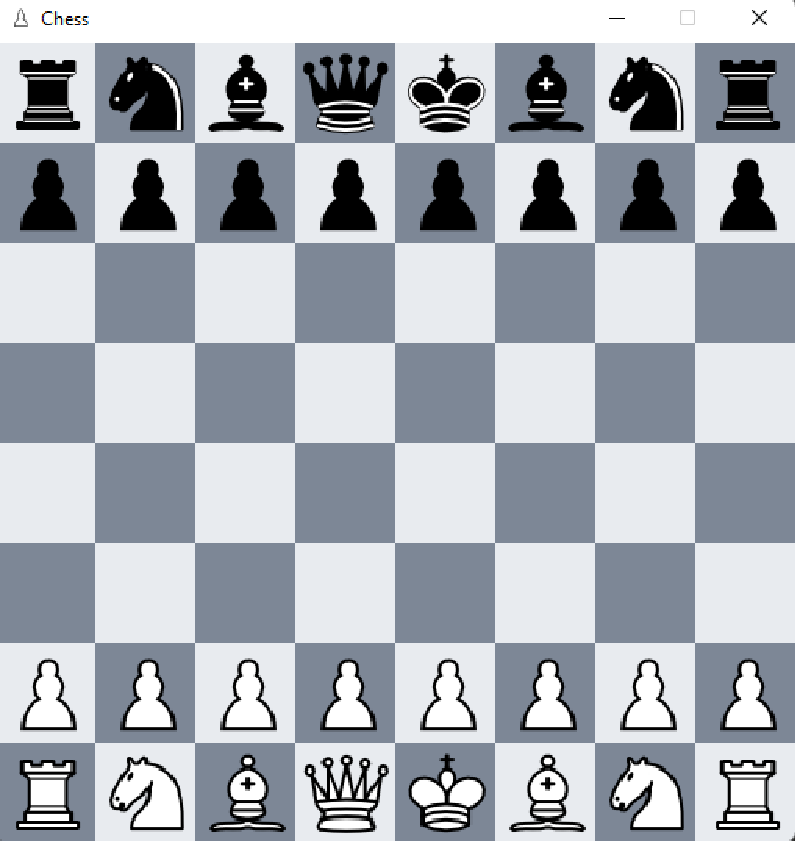
\includegraphics[width=11cm]{frontmatter/figure/scacchiera_gui.pdf}
    \centering
    \caption{Interfaccia grafica vista dall'utente}
    \label{fig:scacchiera_gui}
\end{figure}
\begin{figure}[!htb]
    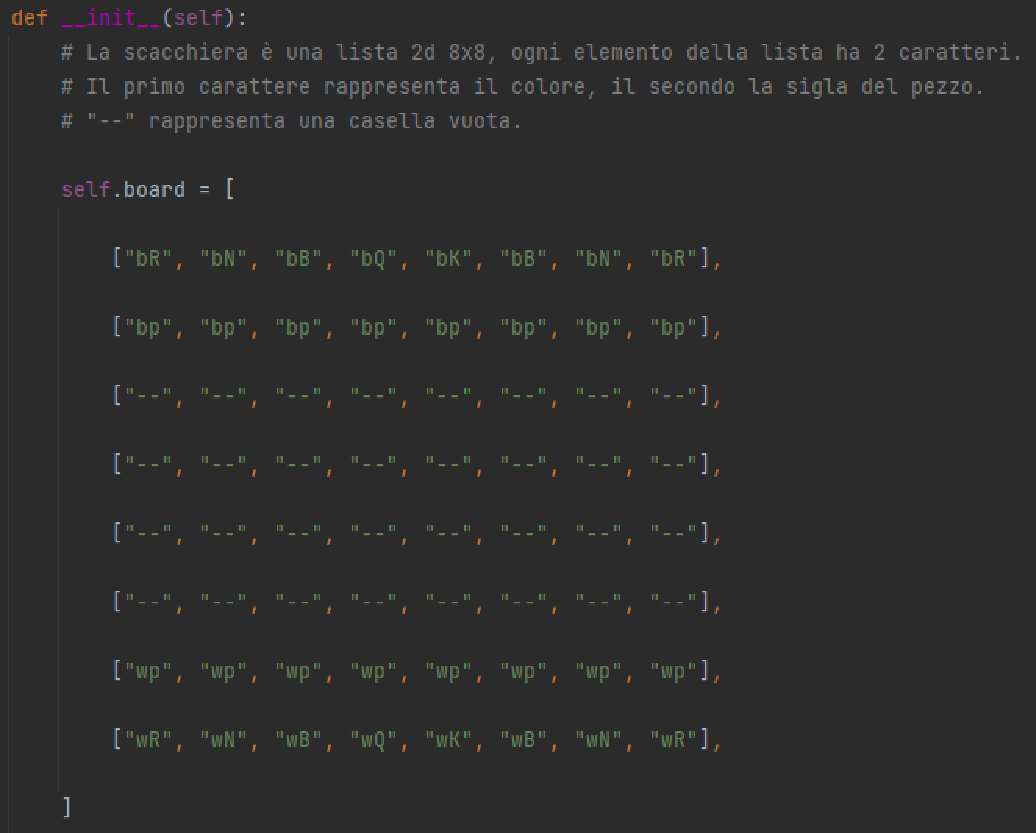
\includegraphics[width=11cm]{frontmatter/figure/rappresentazione_scacchiera.pdf}
    \centering
    \caption{Codifica della figura 3.1}
    \label{fig:rappresentazione_scacchiera}
\end{figure}
\newpage
% Per affiancare due figure
% \begin{figure}[!htb]
% \begin{minipage}[b]{7cm}
% \centering
% 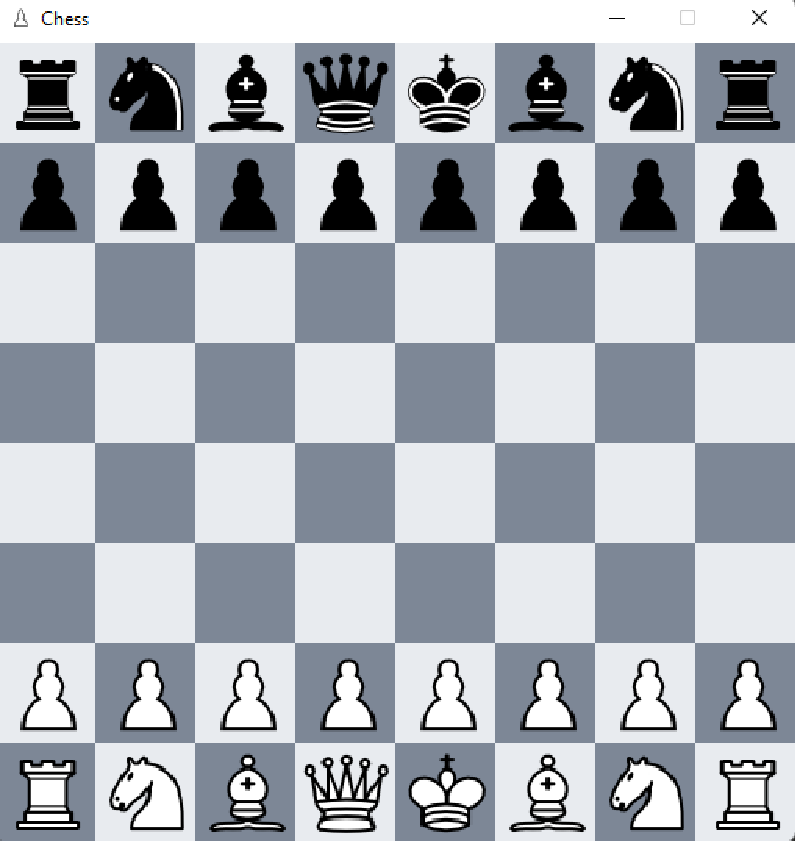
\includegraphics[width=6.5cm]{frontmatter/figure/scacchiera_gui}\\
% \caption{Interfaccia grafica vista dall'utente}
% \label{fig:scacchiera_gui}
% \end{minipage}
% \hspace{1mm}
% \begin{minipage}[b]{7cm}
% \centering
% 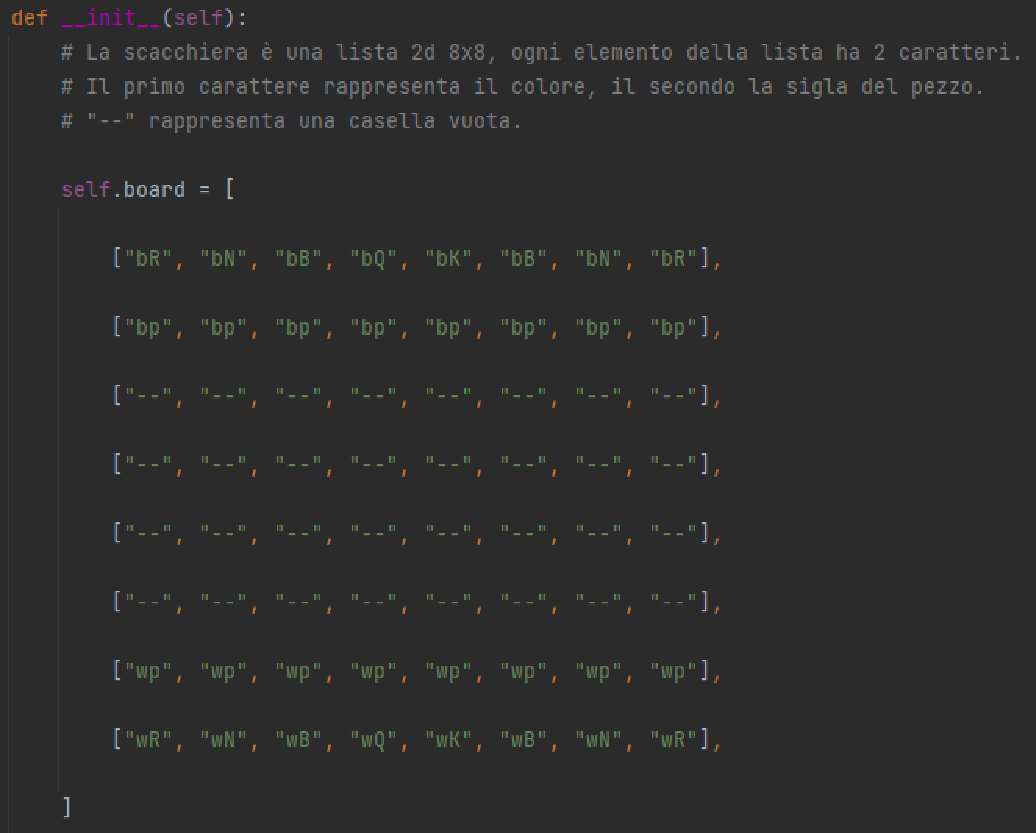
\includegraphics[width=8cm]{frontmatter/figure/rappresentazione_scacchiera}\\
% \caption{Codifica della figura 3.1}
% \label{fig:rappresentazione_scacchiera}
% \end{minipage}
% \end{figure}

A seguito della rappresentazione iniziale della scacchiera sono stati programmati i metodi che si occupano della generazione delle mosse possibili per ciascun pezzo\footnote{Nel gioco degli scacchi il pedone si muove in avanti di una casella (due per la sua prima mossa) e cattura di una casella in diagonale, la torre in orizzontale, l'alfiere in diagonale, il cavallo a L, la regina in orizzontale e in diagonale, e il re di una casella in tutte le direzioni.}, per impedire all'utente di effettuare mosse non legali\footnote{Una mossa non legale è una mossa che pone il re sotto scacco oppure che non libera il re da uno scacco subito nella mossa precedente.}. Analogamente, ad ogni mossa giocata viene effettuato un controllo nel caso in cui il re sia sotto scacco o nel caso in cui vi sia una situazione di scacco matto, dichiarando partita finita nel secondo caso.
\begin{figure}[!htb]
    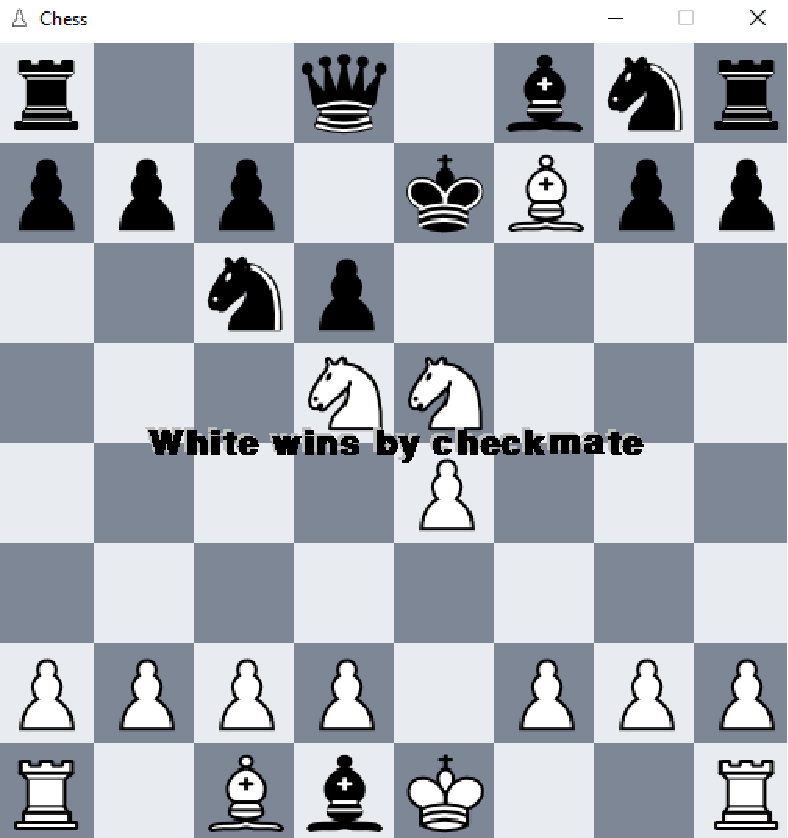
\includegraphics[width=10cm]{frontmatter/figure/checkmate.pdf}
    \centering
    \caption{Partita vinta dal bianco}
    \label{fig:checkmate}
\end{figure}


\subsection{Ricerca delle mosse legali}
Tutta la realizzazione di quanto citato finora è stata effettuata in modo conforme alle tecniche di Intelligenza Artificiale che sono state utilizzate per la generazione delle mosse. L'obiettivo è stato quello di riprogrammare algoritmi di ricerca applicati a una rappresentazione della scacchiera che fosse familiare al programmatore, per comprenderne a fondo il funzionamento. 

\subsubsection{Algoritmo naive}
Una prima, semplice soluzione al problema è stata provata mediante l'utilizzo di un algoritmo naive di ricerca delle mosse. Consideriamo il solito caso in cui il giocatore muove i pezzi bianchi e l'IA i pezzi neri. Dopo una qualsiasi mossa di apertura da parte del bianco, il nero ha un numero molto ristretto di opzioni tra cui scegliere: spostare uno dei pedoni in avanti di una o due caselle, o spostare un cavallo in una delle due caselle legali a inizio partita. Sfruttando un metodo che ritorna la lista di mosse legali data in input una specifica situazione sulla scacchiera, l'algoritmo naive pesca a caso una delle mosse tra quelle disponibili. Chiaramente, un simile approccio sarebbe difficilmente preso in seria considerazione nello sviluppo di un'applicazione del genere, preferendo una soluzione che tenga conto di diversi parametri (mosse storicamente giuste, valore dei pezzi, minacce possibili ai pezzi dell'avversario, trappole in apertura...). Per tale motivo, si è ritenuto necessario lo studio e l'approfondimento di altre metodologie. 

\subsubsection{Algoritmo Greedy}
Nel gioco degli scacchi è fondamentale tenere in considerazione non solo lo stato corrente della scacchiera, ma anche il valore di ciascun pezzo (di solito, un pedone vale molto meno della regina). Sebbene sia vero che talvolta è lo stato stesso della scacchiera a determinare il valore dei pezzi (in alcune situazioni può essere utile sacrificare un pezzo di valore alto per vincere la partita), per convenzione si è deciso di assegnare a ciascun pezzo un valore intero di default. Questi valori sono sfruttati in un metodo di valutazione dello stato corrente della scacchiera, che indica quanto la situazione in corso sia più o meno favorevole per la vittoria.
\begin{figure}[!htb]
    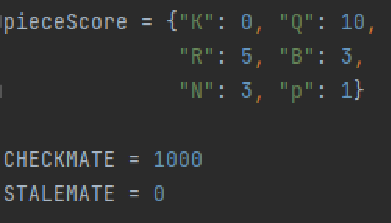
\includegraphics[width=10cm]{frontmatter/figure/valore_pezzi.pdf}
    \centering
    \caption{Valore dei pezzi, scacco matto e stallo}
    \label{fig:valore_pezzi}
\end{figure}\\

Più preciso e affidabile dell'algoritmo precedentemente considerato, l'algoritmo greedy tende più a mettere in difficoltà l'avversario piuttosto che a vincere la partita, spesso in maniera controproducente. La priorità di questa strategia è infatti quella di catturare i pezzi dell'avversario, anche a costo di mettere a rischio i propri. In ogni caso, è interessante notare come, tenendo in considerazione il valore dei pezzi, quest'algoritmo favorisca la cattura di pezzi "pesanti" piuttosto che di altri. 
\subsubsection{Algoritmo minimax}
La strategia minimax è una soluzione studiata appositamente per i giochi a somma zero, come nel caso degli scacchi. Lo scopo, come suggerisce il nome, è quello di \textbf{minimizzare la massima perdita} possibile, analizzando l'albero delle decisioni e valutando l'utilità di un nodo di trovarsi nello stato corrente (a patto che entrambi i giocatori scelgano mosse ottime fino alla fine della partita). A differenza dei due algoritmi precedentemente analizzati, dunque, salta subito all'occhio la prima peculiarità dell'algoritmo, che tiene in stretta considerazione le mosse dell'avversario e gioca comportandosi di conseguenza. Attraverso l'algoritmo minimax il problema di ricerca della mosse migliore è stato ridotto al problema della visita dell'albero delle decisioni. Analizzando la complessità intrinseca del gioco degli scacchi trattata nei capitoli precedenti si è ritenuto necessario effettuare una leggera modifica all'algoritmo minimax che tenesse in considerazione la profondità con cui scendere nell'albero, portando il problema a livelli più o meno trattabili in termini di complessità temporale (l'analisi nel dettaglio delle prestazioni è rimandata al paragrafo \ref{cap: Analisi}).
\subsubsection{Algoritmo negamax con potatura alfa-beta}
% citare wikipedia
L'algoritmo negamax costituisce una variante dell'algoritmo minimax. La caratteristica principale dell'algoritmo è quella di considerare il valore del giocatore A in un certo gioco come la negazione del valore del giocatore B. Così, il giocatore che deve muovere cercherà una mossa che massimizzi la negazione del valore della posizione risultante dalla mossa: così facendo, basta un singolo calcolo per ricavare il valore di tutte le posizioni. Questa è chiaramente una semplificazione rispetto al minimax. Un'ulteriore miglioria all'algoritmo è stata apportata considerando la \textbf{potatura alfa-beta}. L'idea è in realtà applicabile a qualsiasi albero, e consente di ridurre significativamente la complessità di tempo necessaria all'esplorazione. Consideriamo un qualsiasi nodo \textit{n} raggiungibile: se esiste un'alternativa \textit{m} migliore, allora \textit{n} e tutti i suoi discendenti non saranno mai esplorati, portando a una vera e propria "potatura" dell'albero. L'efficacia dell'algoritmo, in ogni caso, dipendente dall'ordinamento dei nodi visitati, che dipende da gioco a gioco. Nel caso degli scacchi, sarebbe una buona idea considerare dapprima le mosse che catturano i pezzi avversari, poi le mosse che li minacciano e infine le altre. 

\subsection{Analisi delle prestazioni}
\label{cap: Analisi}
Non è stata fornita un'analisi delle prestazioni per tutti gli algoritmi discussi finora. Le forti limitazioni di alcune delle strategie adottate per risolvere il problema della ricerca di una mossa non hanno favorito un'interesse significativo: la "casualità" a cui si affida l'algoritmo naive e la bassa considerazione delle mosse dell'avversario dell'algoritmo Greedy non consentirebbero un'indagine interessante. Al contrario, data la natura della strategia minimax che si serve di un vero e proprio albero di ricerca in cui ciascun nodo rappresenta una mossa legale, si è ritenuto opportuno procedere all'analisi prestazionale del suddetto algoritmo. Per sua natura, l'algoritmo minimax non è efficiente in termini di complessità temporale: essendo essa governata dalla dimensione \textit{m} dell'albero, nel caso peggiore la ricerca avrà complessità $O(b^m)$.

\begin{table}[!htb]
    \centering
    \begin{tabular}{|c|c|c|c|}
\hline
\textbf{Profondità} & \textbf{Prima Mossa} & \textbf{Seconda Mossa} & \textbf{Terza Mossa}\\
\hline
\textbf{1} & 0,26 & 0,56 & 0,94\\
\hline
\textbf{2} & 1,39 & 3,02 & 4,02\\
\hline
\textbf{3} & 41,74 & 82,96 & 192,34\\
\hline
\end{tabular}
    \caption{Tempo di visita dell'albero (in secondi) al variare della profondità (senza potatura)}
    \label{tab:my_label}
\end{table}

Tempi del genere rendono il problema intrattabile. Si notano sin da subito, a una profondità non eccessivamente elevata, i tempi d'attesa per la ricerca dopo appena la terza mossa, che in una partita di circa venti o trenta mosse sarebbero notevolmente elevati. Per ovviare al problema è stata aggiunta la tecnica della \textbf{potatura}, che consente di evitare di visitare tutti i nodi dell'albero, alla variante negamax. I risultati delle prestazioni dell'algoritmo negamax con potatura alfa-beta sono forniti di seguito.

\begin{table}[!htb]
    \centering
    \begin{tabular}{|c|c|c|c|}
\hline
\textbf{Profondità} & \textbf{Prima Mossa} & \textbf{Seconda Mossa} & \textbf{Terza Mossa}\\
\hline
\textbf{1} & 0,15 & 0,19 & 0,35\\
\hline
\textbf{2} & 0,86 & 1,32 & 2,85\\
\hline
\textbf{3} & 11,74 & 17,77 & 59,81\\
\hline
\end{tabular}
    \caption{Tempo di visita dell'albero (in secondi) al variare della profondità (con potatura)}
    \label{tab:my_label}
\end{table}

La complessità esponenziale dell'algoritmo permane, ma si può notare dai dati un andamento sostanzialmente "meno esponenziale" dell'algoritmo precedentemente adottato.

\subsection{Migliorie della funzione di valutazione}
A seguito dell'analisi degli algoritmi sono stati effettuati degli esperimenti sul funzionamento delle tecniche di Intelligenza Artificiale apportando modifiche al metodo di valutazione della posizione sulla scacchiera. Come indicato nel paragrafo dedicato all'algoritmo Greedy era stato originariamente considerato un dizionario che tenesse traccia del valore di ciascun pezzo, ottenendo un valore più alto per un pezzo come la Regina piuttosto che per un pedone. Questo paragrafo è invece dedicato alla descrizione di una nuova funzione di valutazione, che tiene traccia non solo del valore di un pezzo, ma anche dell'utilità della sua posizione sulla scacchiera.

\begin{figure}[!htb]
    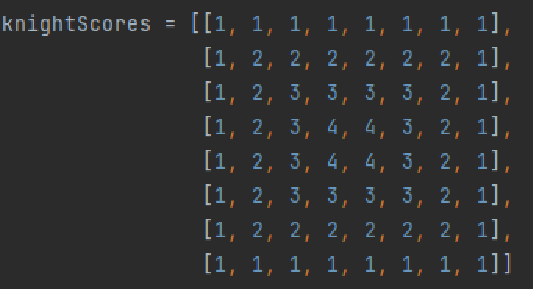
\includegraphics[width=9cm]{frontmatter/figure/cavallo.pdf}
    \centering
    \caption{Utilità delle caselle per il cavallo}
    \label{fig:valore_cavallo}
\end{figure}

\begin{figure}[!htb]
    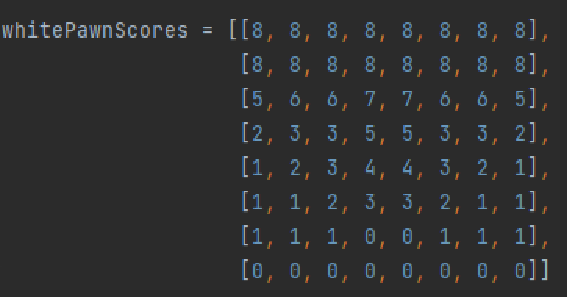
\includegraphics[width=9cm]{frontmatter/figure/pedone.pdf}
    \centering
    \caption{Utilità delle caselle per il pedone bianco}
    \label{fig:valore_pedoni}
\end{figure}
\newpage
Come indicato dalla \textbf{figura \ref{fig:valore_cavallo}} l'utilità del cavallo di trovarsi in una certa casella è stata valutata con un intero da 1 a 4 in base alla "minaccia" che è possibile portare avanti in quella posizione: un cavallo mantenuto verso il centro della scacchiera è chiaramente più forte di un cavallo mantenuto verso i bordi, essendo in quest'ultimo caso più limitato nei movimenti. Analogamente, le posizioni considerate per il pedone bianco nella \textbf{figura \ref{fig:valore_pedoni}} suggeriscono un'idea simile: per un pedone è importante non solo controllare le caselle in diagonale, ma anche cercare di arrivare al lato opposto della scacchiera (al quale è assegnato il valore più alto) per arrivare a promozione. 

\subsubsection{Cambiamenti nelle prestazioni}
Sebbene sia stata apportata una modifica alla funzione di valutazione, la complessità dell'algoritmo di ricerca non è variata in modo significativo. Il motivo è da ricercare, come già spiegato nel paragrafo dedicato, alla natura intrinseca dell'algoritmo. Le costanti migliorie apportate alla funzione di valutazione non sarebbero abbastanza per ridurre i tempi di visita dell'albero delle decisioni. Una riduzione notevole dei tempi di esecuzione era stata già ottenuta attraverso la tecnica della potatura alfa-beta.

\section{Secondo Modulo - Caissa}
La modifica della funzione di valutazione del primo modulo gettava le basi per la ricerca di una metodologia completamente nuova, tenendo a mente le motivazioni e gli obiettivi del lavoro in corso. La volontà di raccogliere i risultati del modulo precedentemente discusso e di evitare di fornire nuovi algoritmi la cui discussione sarebbe stata ridondante si è dunque tradotta nell'intenzione di trattare il problema del gioco degli scacchi da un approccio differente. In questa seconda parte del capitolo si esaminano vere e proprie tecniche di \textbf{Machine Learning}, che sono state sperimentate in un modulo tutto nuovo. I risultati si sono tradotti nella creazione di \textbf{Caissa}, un motore scacchistico in grado di comprendere lo stato della scacchiera e giocare di conseguenza.
\newpage
\subsection{Machine Learning e reti neurali artificiali}
La teoria dell'apprendimento è quella branca dell'Intelligenza Artificiale che si occupa, per l'appunto, dell'apprendimento degli agenti intelligenti, permettendogli di operare in ambienti inizialmente sconosciuti in maniera sempre più appropriata. Tale miglioramento viene effettuato attraverso l'operato stesso dell'agente, dunque in base all'esperienza, ma ciò non preclude necessariamente all'agente di imparare per mezzo di dati che gli sono stati forniti in input.
Uno degli aspetti maggiormente considerati nel contesto analizzato nel lavoro di tesi è quello del \textbf{Deep Learning}: sono state infatti sfruttate tecniche basate su vere e proprie \textbf{reti neurali\footnote{In Biologia, una rete neurale è un gruppo di neuroni che svolgono una determinata funzione fisiologica.} artificiali} organizzate in diversi strati, dove ogni strato scambia le informazioni con quello successivo per garantire un'elaborazione dell'informazione sempre più accurata. Per le tipologie di dati da elaborare le tecniche di Machine Learning adottate si servono di reti neurali \textbf{convoluzionali}, essendo queste particolarmente adatte per l'elaborazione di dati di tipo 2D.

\subsection{Preparazioni preliminari alla fase di addestramento}
Per lo sviluppo del modulo è stata abbandonata l'implementazione precedentemente programmata, favorendo l'utilizzo di una API in linguaggio Python: le esigenze hanno portato alla ricerca di un'implementazione che fosse stabile, completa, e continuamente supportata e manutenuta dagli sviluppatori. Inoltre, è stata utilizzata piattaforma \textbf{Jupyter Notebook}, utile al programmatore per visionare in maniera chiara e user friendly i pezzi sulla scacchiera. Attraverso l'ausilio della piattaforma \textbf{Colab} di Google è stato recuperato il dataset da dare in input al modello di rete neurale per l'addestramento, contenente milioni di partite di scacchi, ciascuna col proprio log delle mosse giocate. L'obiettivo è stato infatti quello di valutare partite note e addestrare il modello a giocare in modo competitivo proprio considerando quelle partite. La valutazione delle posizioni fornite in input è stata effettuata mediante il motore \textit{Stockfish 15} che, sulla base di diversi parametri come ad esempio il vantaggio materiale, la sicurezza del proprio re, la coordinazione dei propri pezzi e diversi altri fattori, fornisce in output un intero positivo (vantaggio del bianco) o negativo (vantaggio del nero).\newpage

\begin{figure}[!htb]
    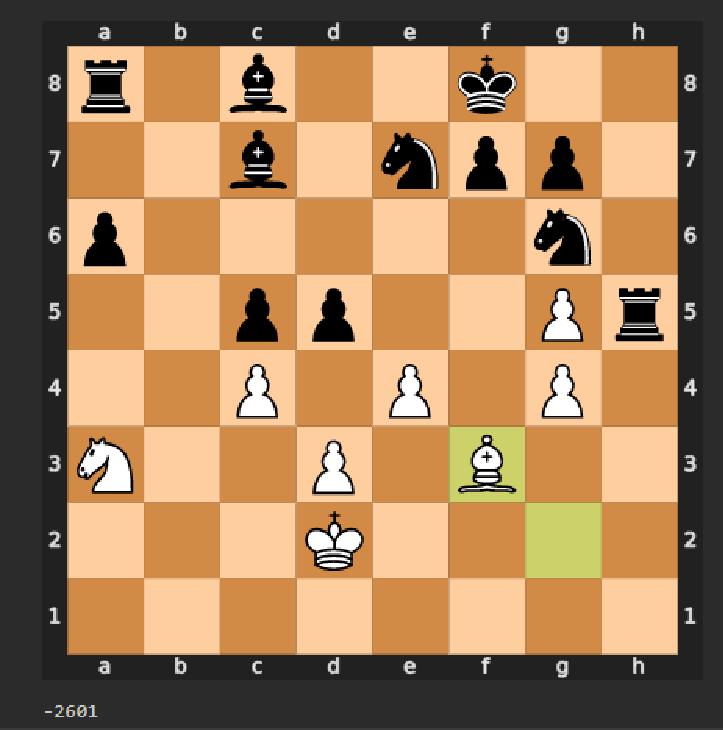
\includegraphics[width=10cm]{frontmatter/figure/valutazione_scacchiera.pdf}
    \centering
    \caption{Vantaggio materiale e posizionale del nero con rispettivo punteggio}
    \label{fig:valutazione_scacchiera}
\end{figure}

La rappresentazione della scacchiera è stata presa e rielaborata per il problema in questione, rendendola più adatta alla rete neurale convoluzionale che sarebbe stata usata in seguito. Nello specifico, è stata adottata una matrice 3D che rappresentasse le caselle e il tipo dei pezzi.

\subsection{Costruzione del modello e addestramento}
Stabiliti gli ambienti favorevoli ha avuto inizio il lavoro vero e proprio, durante il quale Caissa è stato creato e addestrato. Lo sviluppo è avvenuto con \textbf{Keras}, una libreria in Python adatta per l'apprendimento automatico e la creazione di modelli di rete neurale. Dopo aver costruito il tensor sulla base della rappresentazione della scacchiera precedentemente descritta, sono stati aggiunti i layers convoluzionali per la trasmissione delle informazioni. L'addestramento è stato in seguito effettuato sulla base del dataset menzionato nel paragrafo precedente. Infine, è stato implementato un algoritmo minimax di ricerca delle mosse: sebbene si tratti di una soluzione adottata anche nella stesura del primo modulo è interessante notare che, nonostante la differenza di background, la strategia minimax si sia rivelata adatta anche per il funzionamento di un modello di rete neurale.

\subsection{Punteggio ELO e valutazione del modello}
Nell'ambito dei giochi a somma zero è diffuso il metodo di valutazione \textbf{ELO} per calcolare le abilità di un giocatore. Si tratta sostanzialmente di un numero il cui valore aumenta o diminuisce a seconda della vittoria o della sconfitta di una partita contro un altro avversario.
Per la valutazione delle performance di Caissa, dunque, non è stata effettuata un'analisi da un punto di vista computazionale come era stato fatto per il primo modulo. Questo perché eventuali migliorie da apportare a Caissa sarebbero pensate per migliorare la sua performance sportiva: pertanto, è stato scelto un approccio "ad alto livello" sulla base di diverse partite giocate contro altri motori scacchistici preparati dal programmatore. I primi (pochi) incontri sono stati giocati contro il motore \textit{Stockfish 13}. L'intenzione era quella di fissare un upper bound della valutazione di Caissa, essendo \textit{Stockfish} uno dei migliori motori scacchistici moderni con un ELO di circa 3546 alla versione considerata. 
% citare https://www.ichess.net/blog/best-chess-engines/
Come previsto, \textit{Stockfish} ha avuto la meglio in tutte le partite disputate. Partite più eque sono state giocate contro motori scacchistici con un punteggio ELO stimato che varia tra i 500 e i 1200. Nello specifico, sono stati considerati tre modelli: Alpha (512), Beta (870) e Gamma (1190). Nella sua prima versione, in realtà, il punteggio ELO di Caissa è stato stimato al di sotto dei 500 punti, essendo stato battuto persino da Alpha. Nel prossimo capitolo verranno discusse diverse idee che potrebbero essere applicate per migliorare le prestazioni di Caissa e aumentare il suo punteggio.



\newpage

\chapter{Conclusioni} %\label{1cap:spinta_laterale}
% [titolo ridotto se non ci dovesse stare] {titolo completo}
%


\begin{citazione}
	BREVE SPIEGAZIONE CONTENUTO CAPITOLO
\end{citazione}

\newpage

%\part{Impatto ambientale}
\backmatter
\phantomsection
\chapter{Ringraziamenti}
\markboth{Ringraziamenti}{}
% [titolo ridotto se non ci dovesse stare] {titolo completo}
INSERIRE RINGRAZIAMENTI QUI 

% ricordati di ringraziare peppe
\end{document}
